\textbf{Входные параметры:}

 x --- входная переменная (правая граница интегрирования);
 
 Epsilon --- погрешность (например, Epsilon=0.00001).

\textbf{Возвращаемое значение:}

 Значение функции в точке.
 
\textbf{Формула:}
\begin{equation*}
F\left(x \right)=\dfrac{1}{\sqrt{2\pi}}\int_0^x {e^{-\dfrac{x^2}{2}}dx}+0.5, \text{если } x \geq 0.
\end{equation*}
\begin{equation*}
F\left(x \right)=\dfrac{1}{\sqrt{2\pi}}\int_0^{-x} {e^{-\dfrac{-x^2}{2}}dx}+0.5, \text{если } x < 0.
\end{equation*}

 \begin{figure} [h] 
   \center
   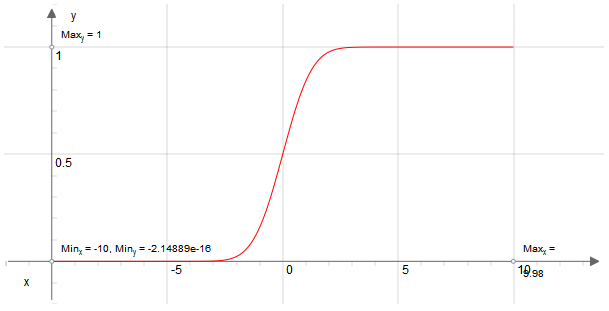
\includegraphics {HML_DistributionFunctionOfNormalizedCenteredNormalDistribution_Graph.png}
   \caption{График функции} 
   \label{img:HML_DistributionFunctionOfNormalizedCenteredNormalDistribution_Graph}  
 \end{figure}
 
